
\section{Investigation of the Radau software applied to the state-dependent discontinuity model}
\label{section:fortran_inaccuracies}
\subsection{Radau}
In this section, we try to solve the state-dependent discontinuity problem with the Fortran solver radau5.f. We investigate how the original Fortran solver deals with the discontinuity. We recall that in both R and Python that `Radau' exhibits an unusual behavior where the solution that is computed does not oscillate between 10000 and 25000 but rather grows exponentially. 

We also note that the event detection in `Radau' in R is added through a C interface and that may explain why Radau in R and Python gives different results when event detection is employed.

We first try the Fortran solver at a tolerance of $10^{-6}$ which is the default in R.
\begin{figure}[h]
\centering
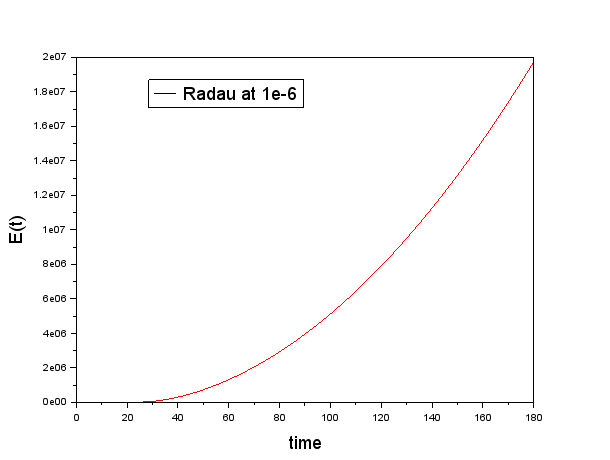
\includegraphics[width=0.7\linewidth]{./figures/fortran_radau_tol_6}
\caption{Solution from the Fortran radau5.f solver at tolerance of $10^{-6}$}
\label{fig:fortran_radau_tol_6}
\end{figure}

From Figure $\ref{fig:fortran_radau_tol_6}$, we again see the unusual behaviour. We also note that it behaves exactly as in R.

We then repeat the process with a tolerance of $10^{-12}$. In Figure $\ref{fig:fortran_radau_tol_12}$, we can see that the computed solution now follows the correct pattern, although it is still not the correct solution that we described in $\ref{subsection:state_with_event_detection}$.

\begin{figure}[h]
\centering
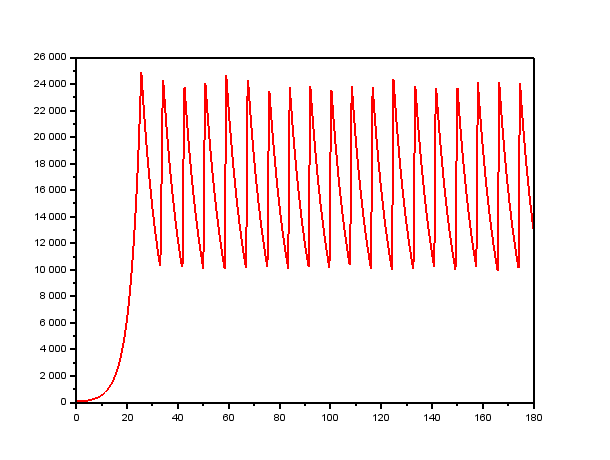
\includegraphics[width=0.7\linewidth]{./figures/fortran_radau_tol_12}
\caption{Solution from the Fortran radau5.f solver at tolerance of $10^{-12}$}
\label{fig:fortran_radau_tol_12}
\end{figure}

From this investigation of the Fortran source code, we can conclude that the issue is not in the interface from R to the Fortran solver or the Python implementation. We also added `print' statements during our investigation to see if the parameter $\beta$ was set to 0.005 which it was. So the problem seems to be with the `Radau' algorithm itself.
